
\section{The choice of streamer}
\label{sec:streamer}
When we got this assignement we had to look at what we would implement in order to test the TRAMP platform. In the sample code there was implemented a simple chat program, so we decided to implement something that streamed a lot of data. There are several ways to do this; we could make a file sharing system, an audio streaming application (like Skype) or a video streaming application. We decided on looking into FFMPEG.

FFMPEG is a complete cross-platform solution to record, convert and stream video and audio. It is a free software licensed under the LGPL or GPL (dependent on the configuration), and is the leading multimedia framework today.\cite{FFMPEG-homepage}
FFMPEG provides tools for converting, streaming, playing and analysing multimedia, as well as a full developers library with the possibility to create allmoast anything you want. Big projects such as QStream, VLC, GStreamer and Google Chrome has used the framework.

Due to time constraints we decided we did not have enough time to implement this framework. Instead we implemented a streamer that copied over one big file by chunking the big file into small bits, sending them and putting them back together on the other side. This will in our eyes show the capabilities of TRAMP just as well as a more sophisticated streamer like the FFMPEG solution we had planned.

\subsection{Our implementation}
To explain what we have done to the code, we must first talk about how the sample chat program work. We decided to use this as a base, as it had a lot of the code we needed anyways. HERE WE MUST TALK ABOUT THE IMPLEMENTATION VINAY DID

\begin{figure*}[ht!]
\centering
 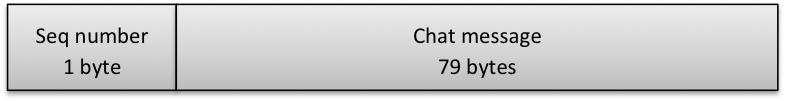
\includegraphics[width=300pt]{sendchatpkt.png}
 % sendchatpkt.png: 786x101 pixel, 150dpi, 13.31x1.71 cm, bb=0 0 377 48
\caption{Packet header for the chat application}
\label{Figure:Packet_header_chat}
\end{figure*}


\begin{figure*}[ht!]
\centering
 
\includegraphics[width=300pt]{sendpkt.png}
 % sendchatpkt.png: 786x101 pixel, 150dpi, 13.31x1.71 cm, bb=0 0 377 48
\caption{Packet header for the file sending addon}
\end{figure*}

